\section{Closed-loop Data-enabled Predictive Control}
This section presents the main result of this article, providing contribution~(\ref{contribution:solves_CL_issue}) whereby we develop \ac{CL-DeePC}. An intuitive explanation is first offered before a proof of the underlying main result is provided.

As a solution to the identification bias that arises in closed-loop due to correlation between inputs and noise %(a demonstration thereof is deferred to Section~\ref{sec:CL_ID_issue})
it is possible to estimate a step-ahead predictor~\citep{Ljung1996}. A prediction horizon length ${f>1}$ is of more practical use in receding horizon optimal control settings, to which end step-ahead predictors can be applied sequentially. 

Fig.~\ref{fig:CL-DeePC} and \eqref{eq:CL_DeePC_no_IVs} illustrate how this idea is employed in \ac{CL-DeePC}. A step-ahead predictor can be obtained from \ac{DeePC} (see Fig.~\ref{fig:regular-DeePC} and \eqref{eq:regular_DeePC_no_IVs}) with $f=1$. In \ac{CL-DeePC} the successive columns of $G$ (from left to right) and their corresponding columns on the right-hand side correspond to sequential applications of \ac{DeePC} with $f=1$ to the same matrix of sufficiently persistently exciting past input-output data on the left-hand side as well as time-shifted windows of input-output data on the right-hand side that encode information on successive initial states.
% \begin{figure}[b!]
% 	\centering
% 	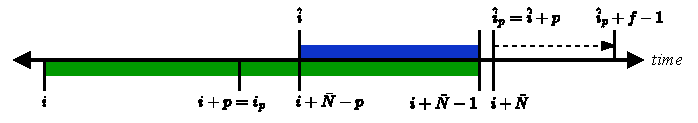
\includegraphics[trim={0.0cm 0.1cm 0.0cm 0.0cm},clip,width=8.4cm]{docs/manuscript/figures/intervals_DeePC.pdf}%[trim={0.0cm 0.0cm 0.0cm 0.0cm},clip,scale=1.0][trim={0.5cm 0.8cm 0.8cm 0.3cm},clip,width=8.4cm]
% 	\caption{Past data from the green ($\datavec{u}{i,\bar{N}},\datavec{y}{i,\bar{N}}$) and blue ($\datavec{u}{\hat{i},p},\datavec{y}{\hat{i},p}$) intervals, shown overlapping as with fully adaptive implementations (for which $i+\bar{N}=\hat{i}_p$), is used to form an output predictor for the black, dashed future prediction window of length $f$. \ac{CL-DeePC} can employ more sample trajectories $N$ of the green window than \ac{DeePC} because its sample trajectories are shorter (due to a shorter prediction window length $f_\mathrm{ID}$ that is used implicitly for identification).}
% 	\label{fig:intervals_DeePC}
% \end{figure}
\subsection{Main result}
To ensure that \ac{CL-DeePC} employs a consistent output predictor the following main result of this article concerns a modification of \eqref{eq:CL_DeePC_no_IVs} that makes use of \ac{IVs}.
\begin{figure}[b!]
\centering
\begin{tikzpicture}
    % defining constants
    \def\stepSize{0.25}
    \def\Nnum{9}
    \def\fnum{8}
    \def\pnum{4}
    
    % Defining lengths
    \newlength{\onelen}
    \setlength{\onelen}{\stepSize cm}
    \newlength{\BrCl}
    \setlength{\BrCl}{0.075cm}
    \newlength{\BrIn}
    \setlength{\BrIn}{0.15cm}
    \newlength{\plen}
    \setlength{\plen}{1cm}%{\pnum\stepSize cm}
    \newlength{\flen}
    \setlength{\flen}{2cm}%{\fnum*\stepSize cm}
    \newlength{\Nlen}
    \setlength{\Nlen}{2.25cm}%{\Nnum\stepSize cm}%should be 2*p+one
    \newlength{\MatClearance}
    \setlength{\MatClearance}{0.3cm}
    
    % grid lines for guidance
    % \draw[gray,step=0.5] (-0,-3) grid (8,3);

    % ======================= drawing data matrix =======================
    \path (0,-\onelen) coordinate (M1A);
    \path ([xshift=\Nlen]M1A) coordinate (M1B);
    \path ([yshift=2*\plen+2*\onelen]M1B) coordinate (M1C);
    \path ([xshift=-\Nlen]M1C) coordinate (M1D);
    \draw[line width=1.5pt] ([xshift=\BrIn,yshift=-\BrCl]M1A) -- ([xshift=-\BrCl,yshift=-\BrCl]M1A) -- ([xshift=-\BrCl,yshift=\BrCl]M1D) -- ([xshift=\BrIn,yshift=\BrCl]M1D); %left bracket
    \draw[line width=1.5pt] ([xshift=-\BrIn,yshift=-\BrCl]M1B) -- ([xshift=\BrCl,yshift=-\BrCl]M1B) -- ([xshift=\BrCl,yshift=\BrCl]M1C) -- ([xshift=-\BrIn,yshift=\BrCl]M1C); %right bracket
    \draw[line width=1pt] ([yshift=\onelen]M1A) -- ([yshift=\onelen]M1B); % dividing matrix into blocks
    \fill[black, opacity=0.5] (M1A) rectangle (M1C);
    \foreach \x in {0,...,8} { % drawing black dots
    \foreach \y in {-1,...,8} {
      \fill ( {(\x+0.5)*\onelen}, {(\y+0.5)*\onelen} ) circle (1pt);
    }}
    \draw[line width=0.1pt] ([yshift=-\plen-\onelen]M1D) -- ([yshift=-\plen-\onelen]M1C);
    \draw[line width=0.1pt] ([yshift=-\plen]M1D) -- ([yshift=-\plen]M1C);

    % coordinates for diagonals
    \path ([yshift=-\plen]M1D) coordinate (M1stair1A);
    \path ([xshift=\plen]M1D) coordinate (M1stair1I);
    % black diagonals
    % \foreach \i in {0,-1}{
    % \foreach \dy in {1,...,11}{
    % \ifthenelse{\dy<5.5}{
    % % This code will be executed if \dy<9.5
    %     \draw[dash pattern=on 1pt off 2pt, line width=0.1pt] ([xshift= 0.5*\onelen,yshift=\i*(\plen+\onelen)-(\dy+0.5)*\onelen]M1D) -- ([xshift= (\dy+0.5)*\onelen,yshift=\i*(\plen+\onelen)-0.5*\onelen]M1D);
    % }{
    % % This code will be executed if \dy>=10
    %     \ifthenelse{\dy<8.5}{
    %         % This code will be executed if \dy<=12
    %         \draw[dash pattern=on 1pt off 2pt, line width=0.1pt] ([xshift= (\dy-3.5)*\onelen,yshift=\i*(\plen+\onelen)-\plen-\onelen+0.5*\onelen]M1D) -- ([xshift=(\dy-8.5)*\onelen,yshift=\i*(\plen+\onelen)-0.5\onelen]M1C);
    %         }{
    %         % This code will be executed if \dy>=13
    %         \draw[dash pattern=on 1pt off 2pt, line width=0.1pt] ([xshift= (\dy-3.5)*\onelen,yshift=(\i-1)*(\plen+\onelen)+0.5\onelen]M1D) -- ([xshift= -0.5*\onelen,yshift=\i*(\plen+\onelen)-(\dy-7.5)*\onelen]M1C);
    %     }
    % }
    % }}
    
    % ---------------- drawing left brace and matrix ----------------
    \path ([xshift=-0.5\BrIn,yshift=-2\BrCl]M1A) coordinate (Brace1L);
    \path ([xshift=0.5\BrIn,yshift=-2\BrCl]M1B) coordinate (Brace1R);
    \draw[decorate, decoration={calligraphic brace, amplitude=3pt, mirror, aspect=0.75},line width=1pt] (Brace1L) -- (Brace1R);
    \node (mat1) at ($(Brace1L)!0.75!(Brace1R) + (0,-3pt)$) {};
    \node[below] at (mat1.center) {$\begin{bmatrix}
        U_{i,p,N}\\U_{i_p,1,N}\\Y_{i,p,N}\\ \hline Y_{i_p,1,N}
    \end{bmatrix}$};
    % brace to the left
    % \path ([xshift=-0.75cm-0.05cm,yshift=-4pt]mat1.center) coordinate (Brace1T);
    % \path ([yshift=-1.73cm]Brace1T) coordinate (Brace1B);
    % \draw[pen colour=gray!60,decorate, decoration={calligraphic brace, amplitude=3pt, mirror, aspect=0.2},line width=0.75pt] (Brace1T) -- (Brace1B);
    % % Zp
    % \node (Zp) at ($(Brace1T)!0.2!(Brace1B) + (-3pt,-0.8pt)$) {};
    % \node[left,text=gray!100,align=center] at ([xshift=0.5mm,yshift=-0.18cm]Zp.center) {\scriptsize{\shortstack{$=$\\$\Phi_{i,1,N}$}}};
  
    % ======================= drawing G =======================
    % useful coordinates
    \path ([xshift=\MatClearance,yshift=\onelen]M1B) coordinate (M2A);
    \path ([xshift=\flen]M2A) coordinate (M2B);
    \path ([yshift=\Nlen]M2B) coordinate (M2C);
    \path ([xshift=-\flen]M2C) coordinate (M2D);

    % brackets
    \draw[line width=1.5pt] ([xshift=\BrIn,yshift=-\BrCl]M2A) -- ([xshift=-\BrCl,yshift=-\BrCl]M2A) -- ([xshift=-\BrCl,yshift=\BrCl]M2D) -- ([xshift=\BrIn,yshift=\BrCl]M2D); %left bracket
    \draw[line width=1.5pt] ([xshift=-\BrIn,yshift=-\BrCl]M2B) -- ([xshift=\BrCl,yshift=-\BrCl]M2B) -- ([xshift=\BrCl,yshift=\BrCl]M2C) -- ([xshift=-\BrIn,yshift=\BrCl]M2C); %right bracket
    
    % red fill
    \fill[red!50,opacity=0.5] (M2A) rectangle (M2C);

    % drawing red dots
    \foreach \x in {0,...,7} {
    \foreach \y in {0,...,8} {
      \fill[red] ([xshift=(\x+0.5)*\onelen,yshift=(\y+0.5)*\onelen]M2A) circle (1pt);%{(\x+0.5)*\onelen+\Nlen+0.5cm}, {(\y+0.5)*\onelen}
    }}

    % dividers
    \foreach \x in {1,...,7}{\draw[line width=0.1pt] ([xshift=\x*\onelen]M2A) -- ([xshift=\x*\onelen]M2D);}

    % drawing middle brace and matrix
    \coordinate (Brace2L) at ([xshift=-0.5\BrIn]M2A |- Brace1L);
    \coordinate (Brace2R) at ([xshift=0.5\BrIn]M2B |- Brace1L);
    \draw[decorate, decoration={calligraphic brace, amplitude=3pt, mirror, aspect=0.5},line width=1pt] (Brace2L) -- (Brace2R);
    \node (mat1) at ($(Brace2L)!0.5!(Brace2R) + (0,-3pt)$) {};
    \node[below] at ([yshift=-0.75cm]mat1.center) {$\underbrace{
    \begin{bmatrix}
        g_1 & g_2 & \cdots & g_f
    \end{bmatrix}}_{= G}$};
    
    % ======================= drawing equal sign ======================= 
    \path ([xshift=\MatClearance*3/4,yshift=\Nlen/2-0.1cm]M2B) coordinate (EqA);
    \path ([xshift=0.4cm]EqA) coordinate (EqB);
    \path ([yshift=0.2cm]EqB) coordinate (EqC);
    \path ([xshift=-0.4cm]EqC) coordinate (EqD);
    \draw[line width = 1.5 pt] (EqA) -- (EqB);
    \draw[line width = 1.5 pt] (EqD) -- (EqC);

    % ---------------- equation sign below ----------------
    \node[below] at ([xshift=5.65\onelen,yshift=-1.05cm]mat1.center) {$=$};

    % ======================= drawing RHS =======================
    % inside of matrix
    \path ([xshift=\MatClearance*3/4,yshift=-\Nlen/2+0.1cm-\onelen]EqB) coordinate (M3A);
    \path ([xshift=\flen]M3A) coordinate (M3B);
    \path ([yshift=2*\plen+2*\onelen]M3B) coordinate (M3C);
    \path ([xshift=-\flen]M3C) coordinate (M3D);
    % top left black triangle
    \path ([yshift=-\plen-\onelen/2]M3D) coordinate (t1A);
    \path ([xshift=\plen+\onelen/2]M3D) coordinate (t1B);
    % top red trapezoid
    \path ([yshift=-\onelen/2]t1A) coordinate (t2A);
    \path ([xshift=\flen]t2A) coordinate (t2B);
    % bottom black triangle
    \path ([yshift=-\plen-\onelen/2]t2A) coordinate (t3A);
    \path ([xshift=\plen+\onelen/2]t2A) coordinate (t3B);
    % bottom red trapezoid
    \path ([yshift=-\onelen/2]t3A) coordinate (t4A);

    % top 'staircase' coordinates
    \path ([yshift=-\plen]M3D) coordinate (stair1A);
    \path ([xshift=\onelen]stair1A) coordinate (stair1B);
    \path ([yshift=\onelen]stair1B) coordinate (stair1C);
    \path ([xshift=\onelen]stair1C) coordinate (stair1D);
    \path ([yshift=\onelen]stair1D) coordinate (stair1E);
    \path ([xshift=\onelen]stair1E) coordinate (stair1F);
    \path ([yshift=\onelen]stair1F) coordinate (stair1G);
    \path ([xshift=\onelen]stair1G) coordinate (stair1H);
    \path ([yshift=\onelen]stair1H) coordinate (stair1I);

    % bottom 'staircase' coordinates
    \path ([yshift=-\onelen]stair1A) coordinate (stair2J);
    \path ([yshift=-\plen]stair2J) coordinate (stair2A);
    \path ([xshift=\onelen]stair2A) coordinate (stair2B);
    \path ([yshift=\onelen]stair2B) coordinate (stair2C);
    \path ([xshift=\onelen]stair2C) coordinate (stair2D);
    \path ([yshift=\onelen]stair2D) coordinate (stair2E);
    \path ([xshift=\onelen]stair2E) coordinate (stair2F);
    \path ([yshift=\onelen]stair2F) coordinate (stair2G);
    \path ([xshift=\onelen]stair2G) coordinate (stair2H);
    \path ([yshift=\onelen]stair2H) coordinate (stair2I);
    
    % fill figures
    % \fill[black, opacity=0.5]  (t1A) -- (t1B) -- (M3D) -- cycle;% top black
    % \fill[red!50, opacity=0.5] (t2A) -- (t2B) -- (M3C) -- (t1B) -- (t1A) -- cycle;% top red
    % \fill[black, opacity=0.5]  (t3A) -- (t3B) -- (t2A) -- cycle;% bottom black
    % \fill[red!50, opacity=0.5] (t4A) -- (M3B) -- (t2B) -- (t3B) -- (t3A) -- cycle; % bottom red
    \fill[black,opacity=0.5]  (M3D) -- (stair1A) -- (stair1B) -- (stair1C) -- (stair1D) -- (stair1E) -- (stair1F) -- (stair1G) -- (stair1H) -- (stair1I) -- cycle;
    \fill[red!50,opacity=0.5] ([xshift=\flen-\onelen]stair1B) -- (stair1B) -- (stair1C) -- (stair1D) -- (stair1E) -- (stair1F) -- (stair1G) -- (stair1H) -- (stair1I) -- (M3C) -- cycle;
    \fill[black,opacity=0.5]  (stair2J) -- (stair2A) -- (stair2B) -- (stair2C) -- (stair2D) -- (stair2E) -- (stair2F) -- (stair2G) -- (stair2H) -- (stair2I) -- cycle;
    \fill[red!50,opacity=0.5] ([xshift=\flen-\onelen]stair2B) -- (stair2B) -- (stair2C) -- (stair2D) -- (stair2E) -- (stair2F) -- (stair2G) -- (stair2H) -- (stair2I) -- ([yshift=-\plen-\onelen]M3C) -- cycle;
    
    % draw brackets
    \draw[line width=1.5pt] ([xshift=\BrIn,yshift=-\BrCl]M3A) -- ([xshift=-\BrCl,yshift=-\BrCl]M3A) -- ([xshift=-\BrCl,yshift=\BrCl]M3D) -- ([xshift=\BrIn,yshift=\BrCl]M3D); %left bracket
    \draw[line width=1.5pt] ([xshift=-\BrIn,yshift=-\BrCl]M3B) -- ([xshift=\BrCl,yshift=-\BrCl]M3B) -- ([xshift=\BrCl,yshift=\BrCl]M3C) -- ([xshift=-\BrIn,yshift=\BrCl]M3C); %right bracket
    
    % U_{i,p,N}
    \path ([xshift=0.5*\onelen,yshift=-\plen+0.5*\onelen]M3D) coordinate (tlbA);
    \foreach \x in {0,...,7}{
    \foreach \y in {0,...,3}{
        \ifthenelse{{\y>\x}\OR{\y=\x}}{%
        % \fill[black, opacity=0.5] ([xshift={(\x-0.5)*\onelen},yshift={(\y-0.5)*\onelen}]tlbA) rectangle ([xshift={(\x+0.5)*\onelen},yshift={(\y+0.5)*\onelen}]tlbA);
        \fill[black] ([xshift={\x*\onelen},yshift={\y*\onelen}]tlbA) circle (1pt);
        }{%
        % \fill[red!50,opacity=0.5] ([xshift={(\x-0.5)*\onelen},yshift={(\y-0.5)*\onelen}]tlbA) rectangle ([xshift={(\x+0.5)*\onelen},yshift={(\y+0.5)*\onelen}]tlbA);%<do this if false>
        \fill[red] ([xshift={\x*\onelen},yshift={(\y*\onelen}]tlbA) circle (1pt);
        }%
    }}
    
    % U_{i_p,1,N}
    \path ([yshift=-\onelen]tlbA) coordinate (tlbB);
    \fill[red!50,opacity=0.5] (stair1A) rectangle ([xshift=\flen,yshift=-\onelen]stair1A);
    \foreach \x in {0,...,7}{\fill[red] ([xshift=\x*\onelen]tlbB) circle (1pt);}
    
    % Y_{i,p,N}
    \path ([yshift=-\plen]tlbB) coordinate (tlbC);
    \foreach \x in {0,...,7}{
    \foreach \y in {0,...,3}{
        \ifthenelse{{\y>\x}\OR{\y=\x}}{%
        \fill[black] ([xshift={\x*\onelen},yshift={\y*\onelen}]tlbC) circle (1pt);%<do this if true>
        }{%
        \fill[red] ([xshift={\x*\onelen},yshift={(\y*\onelen}]tlbC) circle (1pt);%<do this if false>
        }%
    }}

    % Y_{i_p,1,N}
    \path ([yshift=-\onelen]tlbC) coordinate (tlbD);
    \fill[red!50,opacity=0.5] (stair2A) rectangle ([xshift=\flen,yshift=-\onelen]stair2A);
    \foreach \x in {0,...,7}{\fill[red] ([xshift=\x*\onelen]tlbD) circle (1pt);}

    \foreach \dy in {0,-\plen-\onelen}{%
    % black diagonals
    \draw[dash pattern=on 1pt off 2pt, line width=0.1pt] ([xshift= 1/2*\onelen,yshift=\dy+5/2*\onelen]stair1A) -- ([xshift=-5/2*\onelen,yshift=\dy-1/2*\onelen]stair1I);
    \draw[dash pattern=on 1pt off 2pt, line width=0.1pt] ([xshift= 1/2*\onelen,yshift=\dy+3/2*\onelen]stair1A) -- ([xshift=-3/2*\onelen,yshift=\dy-1/2*\onelen]stair1I);
    \draw[dash pattern=on 1pt off 2pt, line width=0.1pt] ([xshift= 1/2*\onelen,yshift=\dy+1/2*\onelen]stair1A) -- ([xshift=-1/2*\onelen,yshift=\dy-1/2*\onelen]stair1I);
    % red diagonals
    \draw[red,dash pattern=on 1pt off 2pt, line width=0.1pt] ([xshift= 1/2*\onelen,yshift=\dy-1/2*\onelen]stair1A) -- ([xshift=1/2*\onelen,yshift=\dy-1/2*\onelen]stair1I);
    \draw[red,dash pattern=on 1pt off 2pt, line width=0.1pt] ([xshift= 3/2*\onelen,yshift=\dy-1/2*\onelen]stair1A) -- ([xshift=3/2*\onelen,yshift=\dy-1/2*\onelen]stair1I);
    \draw[red,dash pattern=on 1pt off 2pt, line width=0.1pt] ([xshift= 5/2*\onelen,yshift=\dy-1/2*\onelen]stair1A) -- ([xshift=5/2*\onelen,yshift=\dy-1/2*\onelen]stair1I);
    \draw[red,dash pattern=on 1pt off 2pt, line width=0.1pt] ([xshift= 7/2*\onelen,yshift=\dy-1/2*\onelen]stair1A) -- ([xshift=7/2*\onelen,yshift=\dy-1/2*\onelen]stair1I);
    \draw[red,dash pattern=on 1pt off 2pt, line width=0.1pt] ([xshift= 9/2*\onelen,yshift=\dy-1/2*\onelen]stair1A) -- ([xshift=7/2*\onelen,yshift=\dy-3/2*\onelen]stair1I);
    \draw[red,dash pattern=on 1pt off 2pt, line width=0.1pt] ([xshift=11/2*\onelen,yshift=\dy-1/2*\onelen]stair1A) -- ([xshift=7/2*\onelen,yshift=\dy-5/2*\onelen]stair1I);
    \draw[red,dash pattern=on 1pt off 2pt, line width=0.1pt] ([xshift=13/2*\onelen,yshift=\dy-1/2*\onelen]stair1A) -- ([xshift=7/2*\onelen,yshift=\dy-7/2*\onelen]stair1I);
    }
    
    % draw dividers
    \draw[line width=0.1pt] ([yshift=-\plen-\onelen]M3D) -- ([yshift=-\plen-\onelen]M3C);
    \draw[line width=0.1pt] ([yshift=-\plen]M3D) -- ([yshift=-\plen]M3C);
    \draw[line width=1pt] ([yshift=\onelen]M3A) -- ([yshift=\onelen]M3B);

    % ---------------- drawing right brace and matrix ----------------
    % brace below matrix
    \path ([xshift=-0.5\BrIn,yshift=-2\BrCl]M3A) coordinate (Brace3L);
    \path ([xshift=0.5\BrIn,yshift=-2\BrCl]M3B) coordinate (Brace3R);
    \draw[decorate, decoration={calligraphic brace, amplitude=3pt, mirror, aspect=0.25},line width=1pt] (Brace3L) -- (Brace3R);
    % matrix below brace
    \node (mat3) at ($(Brace3L)!0.25!(Brace3R) + (0,-3pt)$) {};
    \node[below] at (mat3.center) {$\begin{bmatrix}
        U_{\hat{i},p,f}\\U_{\hat{i}_p,1,f}\\Y_{\hat{i},p,f}\\ \hline \widehat{Y}_{\hat{i}_p,1,f}
    \end{bmatrix}$};
    % tag & label (on RHS of column)
    \node[below] at ([xshift=2.13cm,yshift=-0.9cm]mat3.center) {$\refstepcounter{equation}(\theequation)\label{eq:CL_DeePC_no_IVs}$};
    % brace to the right
    % \path ([xshift=0.7cm+0.05cm]mat3.center |- Brace1T) coordinate (Brace3T);%([xshift=0.7cm,yshift=-4pt]mat3.center) coordinate (Brace3T);
    % \path (Brace3T |- Brace1B) coordinate (Brace3B);
    % \draw[pen colour=gray!60,decorate, decoration={calligraphic brace, amplitude=3pt, aspect=0.2},line width=0.75pt] (Brace3T) -- (Brace3B);
    % % Zf
    % \node (Zf) at ($(Brace3T)!0.2!(Brace3B) + (3pt,-1.5pt)$) {};
    % \node[right,text=gray!100] at ([yshift=-0.18cm]Zf.center) {\scriptsize{\shortstack{$=$\\$\Phi_{\hat{i},1,f}$}}};
    
    % ======================= length indicators ======================= 
    \draw[|-|] ([yshift=\onelen]M1D) -- node[above] {\scriptsize$N$} ([yshift=\onelen]M1C);
    \draw[|-|] ([yshift=\onelen]M2D) -- node[above] {\scriptsize$f$} ([yshift=\onelen]M2C);
    \draw[|-|] ([yshift=\onelen]M3D) -- node[above] {\scriptsize$f$} ([yshift=\onelen]M3C);
    \draw[|-|] ([xshift=\onelen]M3C) -- node[right] {\scriptsize$pr$} ([xshift=\onelen,yshift=\onelen]t2B);
    \draw[|-|] ([xshift=\onelen,yshift=\onelen]t2B) -- node[right] {\scriptsize$r$} ([xshift=\onelen]t2B);
    \draw[|-|] ([xshift=\onelen]t2B) -- node[right] {\scriptsize$pl$} ([xshift=\onelen,yshift=\onelen]M3B);
    \draw[|-|] ([xshift=\onelen,yshift=\onelen]M3B) -- node[right] {\scriptsize$l$} ([xshift=\onelen]M3B);
\end{tikzpicture}
\caption{Visualization of known (black) and unknown (red) variables in \ac{CL-DeePC} without \ac{IVs}. Each dot represents an input $u_k\in\mathbb{R}^r$, output $y_k\in\mathbb{R}^l$, or element of the matrix $G$. \ac{CL-DeePC} involves $f$ sequential applications of a step-ahead predictor obtained from regular \ac{DeePC} with $f=1$ (see also Fig.~\ref{fig:regular-DeePC}), resulting in the dashed block-anti diagonals with the same $u_k$ or $y_k$ on the right hand side.}
\label{fig:CL-DeePC}
\end{figure}
\begin{figure}[b!]
\centering
\begin{tikzpicture}
    % defining constants
    \def\stepSize{0.25}
    \def\Nnum{9}
    \def\fnum{8}
    \def\pnum{4}
    
    % Defining lengths
    % \newlength{\onelen}
    \setlength{\onelen}{\stepSize cm}
    % \newlength{\BrCl}
    \setlength{\BrCl}{0.075cm}
    % \newlength{\BrIn}
    \setlength{\BrIn}{0.15cm}
    % \newlength{\plen}
    \setlength{\plen}{1cm}%{\pnum\stepSize cm}
    % \newlength{\flen}
    \setlength{\flen}{2cm}%{\fnum*\stepSize cm}
    % \newlength{\Nlen}
    \setlength{\Nlen}{2.25cm}%{\Nnum\stepSize cm}%should be 2*p+one
    % \newlength{\MatClearance}
    \setlength{\MatClearance}{0.3cm}
    
    % grid lines for guidance
    % \draw[gray,step=0.5] (-0,-7) grid (8,3);

    % ======================= drawing data matrix =======================
    \path (0,2\plen+\onelen) coordinate (M1D);
    \path ([yshift=-2\plen-2\flen]M1D) coordinate (M1A);
    \path ([xshift=\Nlen]M1A) coordinate (M1B);
    \path ([yshift=2*\plen+2*\flen]M1B) coordinate (M1C);
    \draw[line width=1.5pt] ([xshift=\BrIn,yshift=-\BrCl]M1A) -- ([xshift=-\BrCl,yshift=-\BrCl]M1A) -- ([xshift=-\BrCl,yshift=\BrCl]M1D) -- ([xshift=\BrIn,yshift=\BrCl]M1D); %left bracket
    \draw[line width=1.5pt] ([xshift=-\BrIn,yshift=-\BrCl]M1B) -- ([xshift=\BrCl,yshift=-\BrCl]M1B) -- ([xshift=\BrCl,yshift=\BrCl]M1C) -- ([xshift=-\BrIn,yshift=\BrCl]M1C); %right bracket
    \draw[line width=1pt] ([yshift=\flen]M1A) -- ([yshift=\flen]M1B); % dividing matrix into blocks
    \fill[black, opacity=0.5] (M1A) rectangle (M1C);
    \foreach \x in {0,...,8} { % drawing black dots
    \foreach \y in {-15,...,8} {
      \fill ( {(\x+0.5)*\onelen}, {(\y+0.5)*\onelen} ) circle (1pt);
    }}
    \draw[line width=0.1pt] ([yshift=-\plen-\flen]M1D) -- ([yshift=-\plen-\flen]M1C);
    \draw[line width=0.1pt] ([yshift=-\plen]M1D) -- ([yshift=-\plen]M1C);

    % coordinates for diagonals
    \path ([yshift=-\plen]M1D) coordinate (M1stair1A);
    \path ([xshift=\Nlen]M1D) coordinate (M1stair1I);
    % black diagonals
    % \foreach \i in {0,-1}{
    % \foreach \dy in {1,...,18}{
    % \ifthenelse{\dy<9.5}{
    % % This code will be executed if \dy<9.5
    %     \draw[dash pattern=on 1pt off 2pt, line width=0.1pt] ([xshift= 0.5*\onelen,yshift=\i*(\plen+\flen)-(\dy+0.5)*\onelen]M1D) -- ([xshift= (\dy+0.5)*\onelen,yshift=\i*(\plen+\flen)-0.5*\onelen]M1D);
    % }{
    % % This code will be executed if \dy>=10
    %     \ifthenelse{\dy<12.5}{
    %         % This code will be executed if \dy<=12
    %         \draw[dash pattern=on 1pt off 2pt, line width=0.1pt] ([xshift= 0.5*\onelen,yshift=\i*(\plen+\flen)-(\dy+0.5)*\onelen]M1D) -- ([xshift= -0.5*\onelen,yshift=\i*(\plen+\flen)-(\dy-7.5)*\onelen]M1C);
    %         }{
    %         % This code will be executed if \dy>=13
    %         \draw[dash pattern=on 1pt off 2pt, line width=0.1pt] ([xshift= (\dy-10.5)*\onelen,yshift=\i*(\plen+\flen)-\plen-\flen+0.5*\onelen]M1D) -- ([xshift= -0.5*\onelen,yshift=\i*(\plen+\flen)-(\dy-7.5)*\onelen]M1C);
    %     }
    % }
    % }}
    
    % ---------------- drawing left brace and matrix ----------------
    \path ([xshift=-0.5\BrIn,yshift=-2\BrCl]M1A) coordinate (Brace1L);
    \path ([xshift=0.5\BrIn,yshift=-2\BrCl]M1B) coordinate (Brace1R);
    \draw[decorate, decoration={calligraphic brace, amplitude=3pt, mirror, aspect=0.75},line width=1pt] (Brace1L) -- (Brace1R);
    \node (mat1) at ($(Brace1L)!0.75!(Brace1R) + (0,-3pt)$) {};
    \node[below] at (mat1.center) {$\begin{bmatrix}
        U_{i,p,N}\\U_{i_p,f,N}\\Y_{i,p,N}\\ \hline Y_{i_p,f,N}
    \end{bmatrix}$};
    % brace to the left
    % \path ([xshift=-0.75cm-0.05cm,yshift=-4pt]mat1.center) coordinate (Brace1T);
    % \path ([yshift=-1.73cm]Brace1T) coordinate (Brace1B);
    % \draw[pen colour=gray!60,decorate, decoration={calligraphic brace, amplitude=3pt, mirror, aspect=0.2},line width=0.75pt] (Brace1T) -- (Brace1B);
    % % Zp
    % \node (Zp) at ($(Brace1T)!0.2!(Brace1B) + (-3pt,-0.8pt)$) {};
    % \node[left,text=gray!100,align=center] at ([xshift=0.5mm,yshift=-0.18cm]Zp.center) {\scriptsize{\shortstack{$=$\\$\Phi_{i,f,N}$}}};
  
    % ======================= drawing G =======================
    % useful coordinates
    \path ([xshift=\MatClearance,yshift=-0.5\Nlen-\plen-\flen]M1C) coordinate (M2A);
    \path ([xshift=\onelen]M2A) coordinate (M2B);
    \path ([yshift=\Nlen]M2B) coordinate (M2C);
    \path ([xshift=-\onelen]M2C) coordinate (M2D);

    % brackets
    \draw[line width=1.5pt] ([xshift=0.5\BrIn,yshift=-\BrCl]M2A) -- ([xshift=-\BrCl,yshift=-\BrCl]M2A) -- ([xshift=-\BrCl,yshift=\BrCl]M2D) -- ([xshift=0.5\BrIn,yshift=\BrCl]M2D); %left bracket
    \draw[line width=1.5pt] ([xshift=-0.5\BrIn,yshift=-\BrCl]M2B) -- ([xshift=\BrCl,yshift=-\BrCl]M2B) -- ([xshift=\BrCl,yshift=\BrCl]M2C) -- ([xshift=-0.5\BrIn,yshift=\BrCl]M2C); %right bracket
    
    % red fill
    \fill[red!50,opacity=0.5] (M2A) rectangle (M2C);

    % drawing red dots
    \foreach \x in {0} {
    \foreach \y in {0,...,8} {
      \fill[red] ([xshift=(\x+0.5)*\onelen,yshift=(\y+0.5)*\onelen]M2A) circle (1pt);
    }}

    % drawing middle brace and matrix
    \coordinate (Brace2L) at ([xshift=-0.5\BrIn]M2A |- Brace1L);
    \coordinate (Brace2R) at ([xshift=0.5\BrIn]M2B |- Brace1L);
    \draw[decorate, decoration={calligraphic brace, amplitude=3pt, mirror, aspect=0.5},line width=1pt] (Brace2L) -- (Brace2R);
    \node (mat1) at ($(Brace2L)!0.5!(Brace2R) + (0,-3pt)$) {};
    \node[below] at ([yshift=-1.05cm]mat1.center) {$g$};
    
    % ======================= drawing equal sign ======================= 
    \path ([xshift=\MatClearance*3/4,yshift=\Nlen/2-0.1cm]M2B) coordinate (EqA);
    \path ([xshift=0.4cm]EqA) coordinate (EqB);
    \path ([yshift=0.2cm]EqB) coordinate (EqC);
    \path ([xshift=-0.4cm]EqC) coordinate (EqD);
    \draw[line width = 1.5 pt] (EqA) -- (EqB);
    \draw[line width = 1.5 pt] (EqD) -- (EqC);

    % ---------------- equation sign below ----------------
    \node[below] at ([xshift=2\onelen,yshift=-1.05cm]mat1.center) {$=$};

    % ======================= drawing RHS =======================
    % inside of matrix
    \path ([xshift=0.75\MatClearance]EqB |- M1A) coordinate (M3A);
    \path ([xshift=\onelen]M3A) coordinate (M3B);
    \path ([yshift=2\plen+2\flen]M3B) coordinate (M3C);
    \path ([xshift=-\onelen]M3C) coordinate (M3D);
    
    % fill figures
    \fill[black,opacity=0.5]  (M3D) -- ([yshift=-\plen]M3D) -- ([yshift=-\plen]M3C) -- (M3C) -- cycle;
    \fill[red!50,opacity=0.5] ([yshift=-\plen]M3D) -- ([yshift=-\plen-\flen]M3D) -- ([yshift=-\plen-\flen]M3C) -- ([yshift=-\plen]M3C) -- cycle;
    \fill[black,opacity=0.5] ([yshift=\flen]M3A) -- ([yshift=\flen]M3B) -- ([yshift=\flen+\plen]M3B) -- ([yshift=\flen+\plen]M3A) -- cycle;
    \fill[red!50,opacity=0.5]  (M3A) -- (M3B) -- ([yshift=\flen]M3B) -- ([yshift=\flen]M3A) -- cycle;
    
    % draw brackets
    \draw[line width=1.5pt] ([xshift=0.5\BrIn,yshift=-\BrCl]M3A) -- ([xshift=-\BrCl,yshift=-\BrCl]M3A) -- ([xshift=-\BrCl,yshift=\BrCl]M3D) -- ([xshift=0.5\BrIn,yshift=\BrCl]M3D); %left bracket
    \draw[line width=1.5pt] ([xshift=-0.5\BrIn,yshift=-\BrCl]M3B) -- ([xshift=\BrCl,yshift=-\BrCl]M3B) -- ([xshift=\BrCl,yshift=\BrCl]M3C) -- ([xshift=-0.5\BrIn,yshift=\BrCl]M3C); %right bracket
    
    % U_{i,p,1}
    \foreach \dy in {0,...,-3}{
        \fill[black] ([xshift=0.5\onelen,yshift=(\dy-0.5)*\onelen]M3D) circle (1pt);
    }

    % U_{i_p,f,1}
    \foreach \dy in {-4,...,-11}{
        \fill[red] ([xshift=0.5\onelen,yshift=(\dy-0.5)*\onelen]M3D) circle (1pt);
    }
    
    % Y_{i,p,1}
    \foreach \dy in {0,...,-3}{
        \fill[black] ([xshift=0.5\onelen,yshift=(\dy-0.5)*\onelen-\plen-\flen]M3D) circle (1pt);
    }

    % Y_{i_p,f,1}
    \foreach \dy in {-4,...,-11}{
        \fill[red] ([xshift=0.5\onelen,yshift=(\dy-0.5)*\onelen-\plen-\flen]M3D) circle (1pt);
    }

    % draw dividers
    \draw[line width=0.1pt] ([yshift=-\plen]M3D) -- ([yshift=-\plen]M3C);
    \draw[line width=0.1pt] ([yshift=-\plen-\flen]M3D) -- ([yshift=-\plen-\flen]M3C);
    \draw[line width=1pt] ([yshift=\flen]M3A) -- ([yshift=\flen]M3B);

    % ---------------- drawing right brace and matrix ----------------
    % brace below matrix
    \path ([xshift=-0.5\BrIn,yshift=-2\BrCl]M3A) coordinate (Brace3L);
    \path ([xshift=0.5\BrIn,yshift=-2\BrCl]M3B) coordinate (Brace3R);
    \draw[decorate, decoration={calligraphic brace, amplitude=3pt, mirror, aspect=0.5},line width=1pt] (Brace3L) -- (Brace3R);
    % matrix below brace
    \node (mat3) at ($(Brace3L)!0.5!(Brace3R) + (0,-3pt)$) {};
    \node[below] at ([xshift=0.35cm]mat3.center) {$\begin{bmatrix}
        U_{\hat{i},p,1}\\U_{\hat{i}_p,f,1}\\Y_{\hat{i},p,1}\\ \hline \widehat{Y}_{\hat{i}_p,f,1}
    \end{bmatrix}$};
    % tag & label (on RHS of column)
    \node[below left] at (8.35cm,-5cm) {$\refstepcounter{equation}(\theequation)\label{eq:regular_DeePC_no_IVs}$};
    % brace to the right
    % \path ([xshift=1.1cm]mat3.center |- Brace1T) coordinate (Brace3T);%([xshift=0.7cm,yshift=-4pt]mat3.center) coordinate (Brace3T);
    % \path (Brace3T |- Brace1B) coordinate (Brace3B);
    % \draw[pen colour=gray!60,decorate, decoration={calligraphic brace, amplitude=3pt, aspect=0.2},line width=0.75pt] (Brace3T) -- (Brace3B);
    % % Zf
    % \node (Zf) at ($(Brace3T)!0.2!(Brace3B) + (3pt,-1.5pt)$) {};
    % \node[right,text=gray!100] at ([yshift=-0.18cm]Zf.center) {\scriptsize{\shortstack{$=$\\$\Phi_{\hat{i},f,1}$}}};
    
    % ======================= length indicators ======================= 
    \draw[|-|] ([yshift=\onelen]M1D) -- node[above] {\scriptsize$N$} ([yshift=\onelen]M1C);
    \draw[|-|] ([xshift=\onelen]M3C) -- node[right] {\scriptsize$pr$} ([xshift=\onelen,yshift=-\plen]M3C);
    \draw[|-|] ([xshift=\onelen,yshift=-\plen]M3C) -- node[right] {\scriptsize$fr$} ([xshift=\onelen,yshift=-\plen-\flen]M3C);
    \draw[|-|] ([xshift=\onelen,yshift=-\plen-\flen]M3C) -- node[right] {\scriptsize$pl$} ([xshift=\onelen,yshift=\flen]M3B);
    \draw[|-|] ([xshift=\onelen,yshift=\flen]M3B) -- node[right] {\scriptsize$fl$} ([xshift=\onelen]M3B);
\end{tikzpicture}
\caption{Visualization of known (black) and unknown (red) variables in \ac{DeePC} without \ac{IVs}. Each dot represents an input $u_k\in\mathbb{R}^r$, output $y_k\in\mathbb{R}^l$, or element of the matrix $G$. A multi-step ahead predictor of prediction length $f$ is formed directly by taking a linear combination of past input and output data.\\\vspace{0.75mm}}
\label{fig:regular-DeePC}
\end{figure}
%
% ----------------------------------------------------------- Main result ---------------------------------------------------------------------------------------------
\setcounter{thm}{0}
\begin{thm}\label{theorem:main_result_IVs}
    % Consider the minimal discrete non-deterministic \ac{LTI} system given by~\eqref{eqn:SS_innovation} to generate input-output data in closed-loop with a strictly causal controller. Define data matrices $\Psi_{i,1,N}$ and $\overline{\Psi}_{\hat{i},1,f}$ as in \eqref{eq:Psi_def}. %
    % 
    % If the joint input and noise sequences are sufficiently persistently exciting such that $\left[X_{i,1,N}^\top \; U_{i,p,N}^\top \; U_{i_p,1,N}^\top \; E_{i,p,N}^\top\right]^\top$ is full row rank, and with the choice of \ac{IV} given by $\mathcal{Z}=\Psi_{i,1,N}$ then\\
    Consider the minimal discrete non-deterministic \ac{LTI} system given by~\eqref{eqn:SS_innovation} to generate input-output data in closed-loop by means of a causal controller without direct feedthrough, data matrices $\overline{\Psi}_{\hat{i},1,f}$ and full row rank $\Psi_{i,1,N}$ as in \eqref{eq:Psi_def}, and with an \ac{IV} given by $\mathcal{Z}=\Psi_{i,1,N}$, then\\
    $\mathrm{(i)}$ $\exists G^\mathrm{IV}\in\mathbb{R}^{((p+1)r+pl)\times f}$ such that
    \begin{align}\label{eq:TheoremIV}
        \begin{bmatrix}
            \Psi_{i,1,N}\\Y_{i_p,1,N}
        \end{bmatrix}\mathcal{Z}^\top G^\mathrm{IV} =
        \begin{bmatrix}
            \overline{\Psi}_{\hat{i},1,f}\\\widehat{Y}_{\hat{i}_p,1,f}^\mathrm{IV}
        \end{bmatrix},
    \end{align}
    $\mathrm{(ii)}$ which specifies $\widehat{Y}_{\hat{i}_p,1,f}^\mathrm{IV}$ as an asymptotically unbiased predictor as $p\rightarrow\infty$ and $N\rightarrow\infty$ in accordance with \eqref{eq:relative_rates}. %with respect to future noise and conditioned on past data as $p\rightarrow\infty$, $N\rightarrow\infty$.\\
    %$\mathrm{(iii)}$ that has a variance that is smaller than or equal to the variance of $\widehat{Y}_{\hat{i}_p,1,f}$.
\end{thm}
%
% \begin{thm}\label{theorem:main_result}
%     Consider the minimal discrete non-deterministic \ac{LTI} system given by~\eqref{eqn:SS_innovation} to generate input-output data in closed-loop by means of a causal controller without direct feedthrough, and data matrices $\overline{\Psi}_{\hat{i},1,f}$ and $\Psi_{i,1,N_\mathrm{s}}$ as in \eqref{eq:Phi_def}. If $N_\mathrm{s}=(p+1)r+pl$ such that $\Psi_{i,1,N_\mathrm{s}}$ is square, and furthermore, if $\Psi_{i,1,N_\mathrm{s}}$ is invertible, %
%     %
%     % If the joint input and noise sequences are sufficiently persistently exciting such that $\left[X_{i,1,N}^\top \; U_{i,p,N}^\top \; U_{i_p,1,N}^\top \; E_{i,p,N}^\top\right]^\top$ is full row rank %
%     % ------------------------------------------------------
%     %% ----------------- old version below -----------------
%     %If the input sequence $\{u_k\}_{k=i}^{i+\bar{N}-1}$ of length $\bar{N}=p+s+N-1$ %, with $N\geq(p+s+n)(r+l)+n$ and $p\geq\ell$\todo{don't forget},
%     % is persistently exciting of order $p+s+n$, and has sample correlations such that%
%     % \begin{alignat}{2}%see also https://www.cis.upenn.edu/~jean/schur-comp.pdf
%     % % \widehat{\Sigma}_{u,u} &> 0,\label{eq:PE_corU}\\
%     % &\widehat{\Sigma}_{\mathrm{ee}} - \widehat{\Sigma}_{\mathrm{ue}^\top} \widehat{\Sigma}_{\mathrm{uu}}\inv \widehat{\Sigma}_{\mathrm{ue}}\succ0,\span\span\label{eq:PE_corUE2}\\
%     % &&\text{with}\quad\widehat{\Sigma}_{\mathrm{ee}}&=E_{i,p+s+n,N-n}E_{i,p+s+n,N-n}^\top,\notag\\
%     % &&\widehat{\Sigma}_{\mathrm{ue}}&=U_{i,p+s+n,N-n}E_{i,p+s+n,N-n}^\top,\notag\\
%     % &&\widehat{\Sigma}_{\mathrm{uu}}&=U_{i,p+s+n,N-n}U_{i,p+s+n,N-n}^\top,\notag
%     % \end{alignat}
%     % ------------------------------------------------------
%     then \\
%     $\mathrm{(i)}$ $\exists G\in\mathbb{R}^{N\times f}$ such that
%     \begin{align}\tag{\ref{eq:CL_DeePC_no_IVs}}%\label{eq:Theorem1}
%         \begin{bmatrix}
%             \Psi_{i,1,N_\mathrm{s}}\\
%             Y_{i_p,1,N_\mathrm{s}}
%         \end{bmatrix}G =
%         \begin{bmatrix}
%             \overline{\Psi}_{\hat{i},1,f}\\
%             \widehat{Y}_{\hat{i}_p,1,f}
%         \end{bmatrix},
%     \end{align}
%     $\mathrm{(ii)}$ and with $\widehat{Y}_{\hat{i}_p,1,f}$ as an asymptotically unbiased predictor %with respect to both past and future noise 
%     with respect to future noise and conditioned on past data as $p\rightarrow\infty$.\todo{Compa-rative rates?\\also
%     $N_\mathrm{s}\rightarrow\infty$}%
% \end{thm}

% ----------------------------------------------------------- Auxiliary results ---------------------------------------------------------------------------------------------
\subsubsection{Auxiliary result}
Proof of Theorem~\ref{theorem:main_result_IVs} is deferred till after the following important auxiliary result.
\setcounter{thm}{0}
\begin{lem}\label{lem:relative_rates}\citep{Chiuso2006}
    For scalars $d,\alpha\in\mathbb{R}$, and ${\rho=\max|\emph{eig}(\tilde{A})|<1}$, if the past data window length ${p\rightarrow\infty}$, and the number of columns used to construct block-Hankel data matrices $N\rightarrow\infty$ such that%A necessary condition for consistent closed-loop subspace identification is that as $p\rightarrow\infty$, $N\rightarrow\infty$ such that
    \begin{align}\label{eq:relative_rates}
        \begin{split}
            p &\geq -\frac{d\log N}{2\log|\rho|}, \quad 1 < d < \infty,\\
            p&=o((\log N)^\alpha), \quad \alpha < \infty,%\lim_{p,N\rightarrow\infty} &\; \frac{p}{(\log N)^\alpha}=0, \quad \alpha < \infty,
        \end{split}
    \end{align}
    then errors due to mis-specification of the initial condition are $o_P(1/\sqrt{N})$.
\end{lem}
% For the considered system that was introduced in Section~\secref{sec:sys_model} we have $|\rho|<1$. The conditions formulated by \eqref{eq:relative_rates} are necessary to ensure consistency of the closed-loop estimator because they ensure that errors induced by implicit mis-specification of the initial state are negligible and that sample correlation matrices asymptotically approach well-defined true correlation counterparts \citep{Chiuso2007,Bauer2002}.

% ----------------------------------------------------------- Proof of main result ---------------------------------------------------------------------------------------------
\subsubsection{Proof of Theorem~\ref{theorem:main_result_IVs}}
% ---------------- Proof of (i) ----------------
\noindent\textbf{Proof of $(\mathrm{i})$:} In \eqref{eq:TheoremIV} $G^\mathrm{IV}$ is specified by the top row as
\begin{align}\label{eq:G_sols}
    G^\mathrm{IV} = \left(\Psi_{i,1,N}\mathcal{Z}^\top\right)\inv\overline{\Psi}_{\hat{i},1,f},
\end{align}
where the inverse exists because by choice, $\mathcal{Z}=\Psi_{i,1,N}$, which is full row rank by assumption. $\hfill\qed$
% 
% Decomposing $\Psi_{i,1,N}$ into its dependencies begets
% \begin{align}\label{eq:Phi_isN}
%     \mkern-8mu\Psi_{i,1,N}=\mkern-1mu\begin{bmatrix}
%         U_{i,p,N}\\
%         U_{i_p,1,N}\\
%         Y_{i,p,N}
%     \end{bmatrix}\mkern-1mu=\mkern-1mu
%     \underbrace{\begin{bmatrix}
%         0        & I_{pr} & 0      & 0\\
%         0        & 0      & I_{r} & 0\\
%         \Gamma_p & \mathcal{T}_p^\mathrm{u} & 0 & \mathcal{H}_p
%     \end{bmatrix}}\mkern-3mu\begin{bmatrix}
%         X_{i,1,N}\\
%         U_{i,p,N}\\
%         U_{i_p,1,N}\\
%         E_{i,p,N}
%     \end{bmatrix}\mkern-1mu,
% \end{align}
% in which the matrix on the right hand side is assumed to be full row rank, and the underbraced matrix is also full row rank. Since both of these matrices are full row rank, so is its product $\Psi_{i,1,N}$, meaning that there exists at least one $G$ that satisfies \eqref{eq:CL_DeePC_no_IVs}. 

% \noindent\textbf{Remark 1:} For the matrix on the right hand side of \eqref{eq:Phi_isN} to be guaranteed to be of full row rank a necessary condition is that $N\geq n+(p+1)r+pl$.

% \noindent\textbf{Remark 2:} The full row rank matrix $\Psi_{i,1,N}\in\mathbb{R}^{((p+1)r+pl)\times N}$ has more columns than rows, meaning that in fact there are an infinite number of possibilities for $G$ that satisfy \eqref{eq:CL_DeePC_no_IVs}. These possibilities are given by
% % \begin{align}\label{eq:G_sols}
% %     G = \Psi_{i,1,N}^\dagger\overline{\Psi}_{\hat{i},1,f} + \Pi_{\Psi_{i,1,N}}^\bot W,
% % \end{align}
% in which the dagger $\dagger$ denotes the right inverse ($\mathcal{Q}^\dagger=\mathcal{Q}^\top(\mathcal{Q}\mathcal{Q}^\top)\inv$ with $\mathcal{Q}$ as a real, full row rank matrix), $\Pi_{\Psi_{i,1,N}}^\bot=I_N-\Psi_{i,1,N}^\dagger\Psi_{i,1,N}$ is a projection matrix onto the orthogonal complement of the row space of $\Psi_{i,1,N}$, %see Overschee1996, pg. 19
% and $W\in\mathbb{R}^{N\times f}$ is a matrix of decision variables that parameterizes $G$.

% ---------------- Proof of (ii) ----------------
\noindent\textbf{Proof of $(\mathrm{ii})$:} Applying \eqref{eq:G_sols} to \eqref{eq:TheoremIV} obtains
\begin{align}\label{eq:Yfhat_1}
    \widehat{Y}_{\hat{i}_p,1,f}^\mathrm{IV} = Y_{i_p,1,f}\mathcal{Z}^\top\left(\Psi_{i,1,N}\mathcal{Z}^\top\right)\inv\overline{\Psi}_{\hat{i},1,f}.
\end{align}
Substitution of $Y_{i_p,1,f}$ from \eqref{eq:DataEq2} results in
% Equation \eqref{eq:TheoremIV} stipulates an output predictor as $\widehat{Y}_{\hat{i}_p,1,f}^\mathrm{IV}=Y_{i_p,1,N}\mathcal{Z}^\top G^\mathrm{IV}$. %
% Using \eqref{eq:DataEq1}, \eqref{eq:G_sols}, and considering $\Gamma_1=C$, $\mathcal{H}_1=I_l$, $L_1=\big[C\tKp{u} \;\;\! D \;\;\! C\tKp{y}\big]$ yields
\begin{align}\label{eq:Yfhat_2}
    \begin{split}
        \mkern-6mu\widehat{Y}_{\hat{i}_p,1,f}^\mathrm{IV} = &\bigg(\widetilde{L}_1  + \underbrace{E_{i_p,1,N}\mathcal{Z}^\top}_{=\hat{\Sigma}_{ez}}\big(\underbrace{\Psi_{i,1,N}\mathcal{Z}^\top}_{=\hat{\Sigma}_{\psi z}}\big)\inv\bigg) \overline{\Psi}_{\hat{i},1,f}\\%G^\mathrm{IV}\\
        &+ C \tilde{A}^p X_{i,1,N}\mathcal{Z}^\top G^\mathrm{IV}.
    \end{split}
\end{align}
For $p,N\rightarrow\infty$, in accordance with \eqref{eq:relative_rates}, the initial state contribution is neglecting using Lemma~\ref{lem:relative_rates} since for the considered system $\rho<1$. Moreover, these conditions ensure that the underbraced sample correlations ($\hat{\Sigma}$), approach their well-defined true correlation counterparts~($\Sigma$)~\citep{Chiuso2007,Bauer2002}. With the choice of \ac{IV} of $\mathcal{Z}=\Psi_{i,1,N}$, for the correlation matrix $\hat{\Sigma}_{ez}=\hat{\Sigma}_{e\psi}$ this entails that
\begin{align}\label{eq:E_Phi_correlation}
    \!\!\!\!\begin{split}
        \lim_{\underset{\eqref{eq:relative_rates}}{p,N\rightarrow\infty}}\!\!\hat{\Sigma}_{e\psi} &= \!\lim_{\underset{\eqref{eq:relative_rates}}{p,N\rightarrow\infty}}\frac{1}{N}\;\sum\limits_{k=i_p}^{\mathclap{i_p+N-1}} e_k\!\begin{bmatrix}\datavec{u}{k-p,p+1}^\top & \datavec{y}{k-p,p}^\top \end{bmatrix}\\
        =\Sigma_{e\psi} &=\mathbb{E}\left[e_k\!\begin{bmatrix}\datavec{u}{k-p,p+1}^\top & \datavec{y}{k-p,p}^\top \end{bmatrix}\right]=0.
    \end{split}
\end{align}
The last equality in \eqref{eq:E_Phi_correlation} holds due to the feedback of a (by assumption) strictly causal controller, for which inputs are correlated with preceding noise (${\mathbb{E}[e_k u_j^\top]\neq0,\; \forall j>k}$), but inputs are uncorrelated with concurrent and subsequent noise (${\mathbb{E}[e_k u_j^\top]=0,\; \forall j\leq k}$). Moreover, the innovation noise is then also uncorrelated with preceding outputs (${\mathbb{E}[e_k y_j^\top]=0,\; \forall j<k}$).

By the foregoing analysis, with $\Sigma_{e\psi}=0$ and a vanished initial state contribution, the bias of the predicted output from \eqref{eq:Yfhat_2} w.r.t. the true output from \eqref{eq:DataEq2} is
\begin{align}\label{eq:asym_bias_IV}
    \lim_{\underset{\eqref{eq:relative_rates}}{p,N\rightarrow\infty}}\!\!\mathbb{E}\left[\widehat{Y}_{\hat{i}_p,1,f}^\mathrm{IV}-Y_{\hat{i}_p,1,f}\right]\!=\!\!\lim_{\underset{\eqref{eq:relative_rates}}{p,N\rightarrow\infty}}\!\!\widetilde{L}_1\mathbb{E}\left[\overline{\Psi}_{\hat{i},1,f}-\Psi_{\hat{i},1,f}\right]\!.
\end{align}
The proof of asymptotic unbiasedness is sequential. Note from Fig~\ref{fig:CL-DeePC} that the leftmost columns of $\overline{\Psi}_{\hat{i},1,f}$ and $\Psi_{\hat{i},1,f}$ are equal, so the asymptotic bias of the estimate of this column is zero. Moreover, in combination with \eqref{eq:asym_bias_IV} Fig~\ref{fig:CL-DeePC} shows that the asymptotic bias of subsequent columns to the right is a linear combination of the asymptotic bias of preceding columns to the left. Since the leftmost column is asymptotically unbiased, so are the others in \eqref{eq:asym_bias_IV}. $\hfill\qed$
\setcounter{thm}{0}
\begin{rem}
    Different choices of $\mathcal{Z}$ for which $\Sigma_{\psi z}$ is invertible and $\Sigma_{ez}=0$ are equally valid. The choice of $s=1$ in \eqref{eq:Psi_def} ensures this latter condition with $\mathcal{Z}=\Psi_{i,1,N}$.
\end{rem}
\begin{rem}
    The \ac{IV} used in this proof serves to reduce the number of decision variables as well as to handle noise in such a way as to guarantee the use of a consistent estimator. Without an \ac{IV}, as with \eqref{eq:CL_DeePC_no_IVs}, increasing $N$ both increases the number of decision variables and permits the optimal control problem to select noise in such a way that infeasible trajectories are predicted. As an alternative one may attempt to make the data matrix $\Psi_{i,1,N}$ square and invertible, but then \eqref{eq:relative_rates} is violated in the limit $p,N\rightarrow\infty$ such that the resulting predictor is asymptotically biased.
\end{rem}